%% 
%% Copyright 2007-2020 Elsevier Ltd
%% 
%% This file is part of the 'Elsarticle Bundle'.
%% ---------------------------------------------
%% 
%% It may be distributed under the conditions of the LaTeX Project Public
%% License, either version 1.2 of this license or (at your option) any
%% later version.  The latest version of this license is in
%%    http://www.latex-project.org/lppl.txt
%% and version 1.2 or later is part of all distributions of LaTeX
%% version 1999/12/01 or later.
%% 
%% The list of all files belonging to the 'Elsarticle Bundle' is
%% given in the file `manifest.txt'.
%% 
%% Template article for Elsevier's document class `elsarticle'
%% with harvard style bibliographic references

\documentclass[final, 5p, times, twocolumn, authoryear, 10pt]{elsarticle}

%% Use the option review to obtain double line spacing
%% \documentclass[authoryear,preprint,review,12pt]{elsarticle}

%% Use the options 1p,twocolumn; 3p; 3p,twocolumn; 5p; or 5p,twocolumn
%% for a journal layout:
%% \documentclass[final,1p,times,authoryear]{elsarticle}
%% \documentclass[final,1p,times,twocolumn,authoryear]{elsarticle}
%% \documentclass[final,3p,times,authoryear]{elsarticle}
%% \documentclass[final,3p,times,twocolumn,authoryear]{elsarticle}
%% \documentclass[final,5p,times,authoryear]{elsarticle}
%% \documentclass[final,5p,times,twocolumn,authoryear]{elsarticle}

%% For including figures, graphicx.sty has been loaded in
%% elsarticle.cls. If you prefer to use the old commands
%% please give \usepackage{epsfig}

\usepackage[table,x11names,svgnames,dvipsnames]{xcolor}
\usepackage[export]{adjustbox}
% \usepackage{algorithm}
% \usepackage[noend]{algpseudocode}
\usepackage{amsmath,amssymb,amsfonts}
\usepackage[USenglish]{babel}
\usepackage{bigints}
\usepackage{bm}
\usepackage{booktabs}
\usepackage{cancel}
\usepackage[tableposition=above, font=normalsize]{caption}
% \usepackage{centernot}
% \usepackage{comment}
\usepackage{empheq}
\newcommand*\widefbox[1]{\fbox{\hspace{2em}#1\hspace{2em}}}
\usepackage{enumitem}
\usepackage{epsfig}
\usepackage{epstopdf}
% \epstopdfsetup{outdir=./figures//}
% \usepackage[letterpaper, top=1.0in, bottom=1.0in, left=1.0in, right=1.0in]{geometry}
\RequirePackage[OT1]{fontenc}
% \usepackage{fontspec}
\usepackage{graphics}
\usepackage{graphicx}
\graphicspath{{../figures/}}
% \usepackage{ifpdf}
% \usepackage{lastpage}
% \usepackage{leftidx}
\usepackage{lineno}
\usepackage{lipsum}
% \usepackage{mathrsfs}
\usepackage{mathtools}
\usepackage{multicol}
\usepackage{multirow}
\usepackage{nicefrac}
% \usepackage{nicematrix}
% \usepackage{pgfplots}
\usepackage{pifont}
% \usepackage{ragged2e}
% \usepackage{rotating}
% \usepackage{stmaryrd}
\usepackage{siunitx}
\usepackage{soul}
\usepackage[caption=false]{subfig}
\usepackage{tabularx}
\usepackage{threeparttable}
\usepackage{tikz}
% \usepackage{tkz-euclide}
% \usepackage{ctable}
% \usetikzlibrary{matrix, arrows}
\usetikzlibrary{shapes.geometric, arrows, decorations.markings, shapes.arrows}

\newcommand{\minitab}[2][l]{\begin{tabular}{#1}#2\end{tabular}}

%%%%%%% TODO NOTES 
\usepackage{todonotes}
\setlength{\marginparwidth}{1.3cm}
\setlength{\marginparsep}{0cm}
\newcommand{\ctodo}[1]{\todo[size=\tiny]{#1}}
\newcommand{\nnparam}{\theta}
\newcommand{\pinn}{\pi_{\nnparams}}

\usepackage{ulem}
\usepackage{wrapfig}

\tikzstyle{startstop} = [rectangle, rounded corners, minimum width=1cm, minimum
height = 0.5cm, text centered, draw=black, fill=red!30]
\tikzstyle{io} = [trapezium, trapezium left angle=70, trapezium right angle=110,
minimum height=1cm, text width=3cm, text centered, draw=black, fill=blue!30]
\tikzstyle{process} = [rectangle, minimum width=2cm, minimum height=0.8cm, text
centered, text width=2cm, draw=black, fill=orange!30]
\tikzstyle{decision} = [diamond, aspect=1.25, minimum width=2cm, minimum height=0.5cm, 
text centered, text width=3cm, draw=black, fill=green!30]
\tikzstyle{arrow} = [thick, ->, >=stealth]




\makeatletter
\newcommand{\rmnum}[1]{\romannumeral #1}
\newcommand{\Rmnum}[1]{\expandafter\@slowromancap\romannumeral #1@}
\makeatother

\DeclarePairedDelimiter\ceil{\lceil}{\rceil}
\DeclarePairedDelimiter\floor{\lfloor}{\rfloor}

\newcommand{\bmat}[1]{\begin{bmatrix}#1\end{bmatrix}}
\newcommand{\pmat}[1]{\begin{pmatrix}#1\end{pmatrix}}
\newcommand{\ubar}[1]{\text{\b{$#1$}}}
\newcommand{\norm}[2]{\|{#1}\|_{{}_{#2}}}
\newcommand{\abs}[1]{\left|{#1}\right|}
\newcommand{\mbf}[1]{\mathbf{#1}}
\newcommand{\mc}[1]{\mathcal{#1}}
\newcommand{\dd}{\operatorname{d}\!}
\newcommand{\muc}[2]{\multicolumn{#1}{c}{#2}}
\newcommand*\Eval[3]{\left.#1\right\rvert_{#2}^{#3}}
\newcommand{\inner}[1]{\left\langle#1\right\rangle}
\newcommand{\pd}[2]{\frac{\partial #1}{\partial #2}}
\newcommand{\pdd}[2]{\frac{\partial^2 #1}{\partial #2^2}}
\newcommand{\el}[2]{\frac{\dd}{\dd t}\pd{\mc{L}}{\dot{#1}} - \pd{\mc{L}}{#1} = #2}
\newcommand{\elk}[2]{\frac{\dd}{\dd t}\pd{\mc{L}}{\dot{#1}_k} - \pd{\mc{L}}{#1_k} = #2_k}
\newcommand{\vectornorm}[1]{\left|\left|#1\right|\right|}
\newcommand{\dom}[1]{\textrm{dom}\;#1}
\newcommand{\bx}{{\bf x}}
\newcommand{\bu}{{\bf u}}
\newcommand{\cmark}{\ding{51}}%
\newcommand{\xmark}{\ding{55}}%
\newcommand*{\vertbar}{\rule[-1ex]{0.5pt}{2.5ex}}
\newcommand*{\horzbar}{\rule[.5ex]{2.5ex}{0.5pt}}

\newcommand{\idapbc}{\textsc{IdaPbc}}
\newcommand{\electric}{{\textcolor{blue}{\hspace{-0.5mm}$\bm{E}$\;}}}
\newcommand{\magnetic}{{\textcolor{red}{\hspace{-0.5mm}$\bm{B}$\;}}}

% \theoremstyle{plain}
% \newtheorem{thm}{Theorem}[section]
\newtheorem{thm}{Theorem}
% \makeatletter
% \@addtoreset{thm}{section}
% \makeatother
% \newtheorem{cor}[thm]{Corollary}
\newtheorem{lem}{Lemma}
% \newtheorem{claim}[thm]{Claim}
% \newtheorem{axiom}[thm]{Axiom}
% \newtheorem{conj}[thm]{Conjecture}
% \newtheorem{fact}[thm]{Fact}
% \newtheorem{hypo}[thm]{Hypothesis}
% \newtheorem{assum}[thm]{Assumption}
\newtheorem{prop}{Proposition}
% \newtheorem{crit}[thm]{Criterion}
% \theoremstyle{definition}
\newtheorem{defn}[thm]{Definition}
% \newtheorem{exmp}[thm]{Example}
\newtheorem{rem}{Remark}
% \newtheorem{prin}[thm]{Principle}

\DeclareMathOperator{\Tr}{tr}
\newcommand\xdownarrow[1][2ex]{%
   \mathrel{\rotatebox{90}{$\xleftarrow{\rule{#1}{0pt}}$}}
}
\DeclareMathOperator{\End}{End}
\DeclareMathOperator{\Hom}{Hom}
\DeclareMathOperator{\id}{id}
\DeclareMathOperator{\vers}{vers}
\DeclareMathOperator{\trans}{Trans}
\DeclareMathOperator{\rot}{Rot}
\DeclareMathOperator{\rank}{rank}
\DeclareMathOperator{\sinc}{sinc}

\usepackage{hyperref}
\hypersetup{
    unicode=false,          % non-Latin characters in Acrobat’s bookmarks
    pdftoolbar=true,        % show Acrobat’s toolbar?
    pdfmenubar=true,        % show Acrobat’s menu?
    pdffitwindow=false,     % window fit to page when opened
    pdfstartview={FitH},    % fits the width of the page to the window
    pdftitle={Mischievous Sibling's Grid World},    % title
    pdfauthor={Aykut C. Satici}, % author
    % pdfsubject={Subject},   % subject of the document
    % pdfcreator={Creator},   % creator of the document
    % pdfproducer={Producer}, % producer of the document
    % pdfkeywords={keyword1, key2, key3}, % list of keywords
    pdfnewwindow=true,      % links in new PDF window
    colorlinks=true,       % false: boxed links; true: colored links
    linkcolor=blue!30!green,          % color of internal links (change box color with linkbordercolor)
    linkbordercolor=orange,
    citecolor=blue,        % color of links to bibliography
    citebordercolor=green,
    filecolor=magenta,      % color of file links
    urlcolor=cyan,           % color of external links
    urlbordercolor=blue,
}


\journal{Convoluted Questions (Dolamba\c{c}l\i{} Sorular)}

\begin{document}


\begin{frontmatter}

%% Title, authors and addresses

%% use the tnoteref command within \title for footnotes;
%% use the tnotetext command for theassociated footnote;
%% use the fnref command within \author or \affiliation for footnotes;
%% use the fntext command for theassociated footnote;
%% use the corref command within \author for corresponding author footnotes;
%% use the cortext command for theassociated footnote;
%% use the ead command for the email address,
%% and the form \ead[url] for the home page:
%% \title{Title\tnoteref{label1}}
%% \tnotetext[label1]{}
%% \author{Name\corref{cor1}\fnref{label2}}
%% \ead{email address}
%% \ead[url]{home page}
%% \fntext[label2]{}
%% \cortext[cor1]{}
%% \affiliation{organization={},
%%            addressline={}, 
%%            city={},
%%            postcode={}, 
%%            state={},
%%            country={}}
%% \fntext[label3]{}

\title{Mischievous Sibling's Grid World}

%% use optional labels to link authors explicitly to addresses:
%% \author[label1,label2]{}
%% \affiliation[label1]{organization={},
%%             addressline={},
%%             city={},
%%             postcode={},
%%             state={},
%%             country={}}
%%
%% \affiliation[label2]{organization={},
%%             addressline={},
%%             city={},
%%             postcode={},
%%             state={},
%%             country={}}

\author[label1]{Aykut C. Satici}
\ead{aykutsatici@boisestate.edu}

% \author[label2]{Gokhan Atinc}
% \ead{gokhan.atinc@mathworks.com}

%Department and Organization
\affiliation[label1]{organization={Boise State University},
            addressline={Mechanical and Biomedical Engineering}, 
            city={Boise},
            postcode={83725}, 
            state={Idaho},
            country={USA}}

\cortext[cor1]{Corresponding author}

% \affiliation[label2]{organization={Mathworks Inc.},
%             addressline={1 Lakeside Campus Drive}, 
%             city={Natick},
%             postcode={01760}, 
%             state={Massachusetts},
%             country={USA}}

\begin{abstract}
    % This is a technical note solving an interesting question posed by a friend
    % and colleague, G\"{o}khan At{\i}n\c{c}. 
    This is a technical note that introduces a novel grid world environment and
    an optimal control problem that is meant to be solved by a reinforcement
    learning (RL) agent in one-shot. That is to say, the algorithm that the RL
    agent runs is supposed to be able to solve the environment by training only
    for a single episode. The environment is very similar to the well-known Grid
    World problem, but with a twist. We solve the problem in two different ways:
    first using a direct probability calculation and then using reinforcement
    learning on a judiciously designed Markov Decision Process. The results are
    compared and discussed. The numerical solution to the problem allows us to 
    provide further statistics that sheds some more insight into the problem.
\end{abstract}

% %%Graphical abstract
% \begin{graphicalabstract}
% %\includegraphics{grabs}
% \end{graphicalabstract}
% 
% 
% %%Research highlights
% \begin{highlights}
% \item Research highlight 1
% \item Research highlight 2
% \end{highlights}


\begin{keyword}
Probability \sep Expectations \sep Reinforcement learning \sep Gymnasium \sep
Policy iteration 

% \JEL C45 \sep C53 \sep C55 \sep C82 \sep F47 \sep O50
%% keywords here, in the form: keyword \sep keyword
%% PACS codes here, in the form: \PACS code \sep code
%% MSC codes here, in the form: \MSC code \sep code
%% or \MSC[2008] code \sep code (2000 is the default)
\end{keyword}


\end{frontmatter}

% \linenumbers
%% main text
\section{Introduction}
\label{sec:intro}
%
The question is interesting and the solutions are just as interesting. Let us 
delve right into it.
\vspace{-1mm}
\section{Problem Statement}
%
% \begin{wrapfigure}{r}{0.4\textwidth} %this figure will be at the right
%     \vspace{-5mm}
%     \centering
%     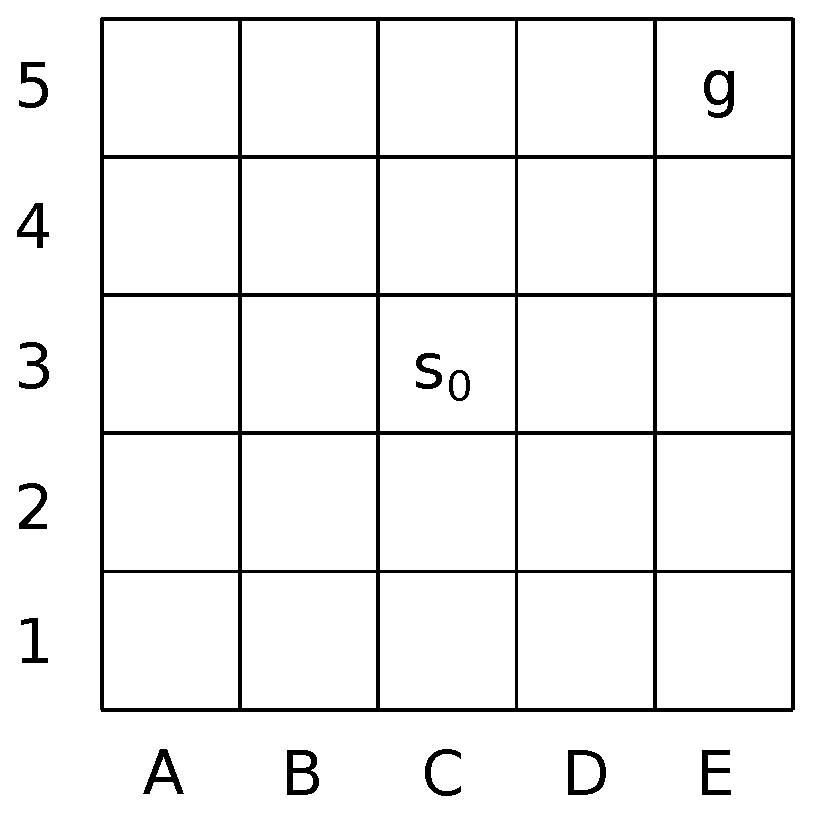
\includegraphics[width=0.25\textwidth]{./figures/drawing.eps}
%     \caption{Problemin \c{s}emati\u{g}i}
%     \label{fig:schematic}
%     \vspace{-5mm}
% \end{wrapfigure}
%
\begin{minipage}{0.5\textwidth}
    Consider the blue rectangle that shares its bottom left corner with that of
    the triangle $\triangle ABC$ as seen in the figure to the right. The length
    of the line segment between points $B$ and the top left corner of the
    rectangle is $4$ units while the length of the line segment between the
    bottom right corner of the rectangle and point $C$ is $3$  units.
\end{minipage}
\begin{minipage}{0.5\textwidth}
\begin{tikzpicture}[scale=0.85]
\tkzInit[xmax=8, ymax=8/3]
% \tkzDefPoint(0,0){B}
\tkzDefPoint(0,0){A}
\tkzDefPoint(8,0){C}
\tkzDrawTriangle[two angles = 90 and 18.43494882292201](A,C)
\tkzGetPoint{B}
\tkzLabelPoints[below left](A)
\tkzLabelPoints[below right](C)
\tkzLabelPoints[above left](B)

\tkzDefPoint(0,1){D}
\tkzDefPoint(5,0){E}
\tkzDefPoint(5,1){F}
\tkzDrawPolygon[fill=black!50!blue!20!, opacity=0.75](A,D,F,E)
% \tkzLabelPoints[below](E)
% \tkzLabelPoints[left](D)

\tkzMarkRightAngles(C,A,tkzPointResult)
\tkzDrawPoints(A,B,C)

\tkzDefPoint(5,-0.1){E1}
\tkzDefPoint(5,-0.3){E2}
\tkzDrawSegment[color=black](E1,E2)
\tkzDefPoint(8,-0.1){C1}
\tkzDefPoint(8,-0.3){C2}
\tkzDrawSegment[color=black](C1,C2)
\tkzDefMidPoint(E1,E2) \tkzGetPoint{E12mid}
\tkzDefMidPoint(C1,C2) \tkzGetPoint{C12mid}
\tkzDrawSegment[color=black](E12mid,C12mid)

\tkzDefPoint(-0.1,8/3){B1}
\tkzDefPoint(-0.3,8/3){B2}
\tkzDrawSegment[color=black](B1,B2)
\tkzDefPoint(-0.1,1){D1}
\tkzDefPoint(-0.3,1){D2}
\tkzDrawSegment[color=black](D1,D2)
\tkzDefMidPoint(B1,B2) \tkzGetPoint{B12mid}
\tkzDefMidPoint(D1,D2) \tkzGetPoint{D12mid}
\tkzDrawSegment[color=black](B12mid,D12mid)

\tkzLabelSegment[left, font=\footnotesize](B12mid,D12mid){4}
\tkzLabelSegment[below, font=\footnotesize](E12mid,C12mid){3}

\end{tikzpicture}
\end{minipage}

\begin{enumerate}
    \setlength\itemsep{0em}
    \item Find the area of the rectangle.
    \item What is the minimum area of the triangle $\triangle ABC$?
\end{enumerate}
\section{Solutions}
\label{sec:solutions}
%
We present two solutions to the problem: a probabilistic solution and a
reinforcement learning (RL) solution.

\subsection{Probability Solution}
\label{ssec:prob_sol}
%
We invoke a celebrated theorem from probability theory that will help us solve
the problem. This theorem is called the \textit{law of total expectation} or
\textit{tower rule of probability theory} in the
literature~\cite{bertsekas2002introduction}.
%
In this section, we use the correspondence $\{1, 2, 3, 4, 5\} \mapsto \{0, 1, 2,
3, 4\}$ and $\{A, B, C, D, E\} \mapsto \{0, 1, 2, 3, 4\}$ for legacy reasons.
%
\begin{thm}[Tower rule] \label{thm:tower} Let $X$ be a random variable and
    $\{A_i\}_i^m$ be a finite partition of the sample space. Then, 
    \[ \mathbb{E}[X] = \sum_i^m \mathbb{E}\left[ X \mid A_i \right]
    \mathbb{P}(A_i). \]
\end{thm}
%
We denote the square on which the robot resides at the $k^{\text{th}}$ step by
$s_k$ and the goal square by $g$. Consider the following family of random
variables.
\begin{equation}
    C_n := \sum_{k=n+1}^\infty r_k, \qquad r_k = 
\begin{cases}
    1 & \mbox{if } s_k \neq g \\
    0 & \mbox{if } s_k = g
\end{cases}.
\label{eq:RVs}
\end{equation}
%
The sum in this definition is well-defined because once the robot reaches $g$,
all the remaining $r_k$'s take the value zero. We are being asked the value of
$\mathbb{E}[C_0]$. To that end, we will use the following repercussion of
definition~\eqref{eq:RVs}.
% \vspace{-2mm}
\begin{equation*} 
    C_m = \sum_{i=m+1}^n r_i + C_n, \qquad m \leq n.
\end{equation*}
% \vspace{-3mm}
% Beklenen de\u{g}erin \"{o}zelliklerini kullanarak a\c{s}a\u{g}{\i}daki sonuca
% varabiliriz.
Using the properties of expectation, if $s_i \neq g$ for $m < i < n$, we can
deduce the following result.
% \vspace{-1mm}
\begin{equation*} 
    \mathbb{E}[C_m] = \sum_{i=m+1}^n \mathbb{E}[r_i] + \mathbb{E}[C_n] = n-m + \mathbb{E}[C_n].
    % \begin{cases}
    %     k + \mathbb{E}[C_n] & \mbox{e\u{g}er } s_i \neq g \\
    %     \mathbb{E}[C_n] & \mbox{e\u{g}er } s_i = g
    % \end{cases}, 
    % \qquad m < i < n, \;\; s_i \neq g.
\end{equation*}
%
Using the properties of expectation, if $s_i \neq g$ for $m < i < n$, we can
deduce the following result.
%
\begin{equation*} 
    \mathbb{E}[C_m] = \sum_{i=m+1}^n \mathbb{E}[r_i] + \mathbb{E}[C_n] = n-m + \mathbb{E}[C_n].
    % \begin{cases}
    %     k + \mathbb{E}[C_n] & \mbox{e\u{g}er } s_i \neq g \\
    %     \mathbb{E}[C_n] & \mbox{e\u{g}er } s_i = g
    % \end{cases}, 
    % \qquad m < i < n, \;\; s_i \neq g.
\end{equation*}
%
Similar identities to the above expression hold for conditional expectations as
well. Using the tower rule~\ref{thm:tower}, we start to compute.
% %
\begin{align}
   \begin{split}
    \mathbb{E}[C_0] &= \mathbb{E}\left[ C_0 \mid s_1 \in \{C4, D3\} \right] 
    \underbrace{\mathbb{P}(s_1 \in \{C4, D3\})}_{=\frac{1}{2}} \\ 
    &+
    \mathbb{E}\left[ C_0 \mid s_1 \in \{B3, C2\} 
    \right] \underbrace{\mathbb{P}(s_1 \in \{B3, C2\})}_{=\frac{1}{2}}.
    \end{split}
    \label{eq:tower1}
\end{align}
%
From now on, we will assume $s_1 = C4$ in the first term on the right-hand side
and $s_1 = C2$ in the second. Notice that, because of the inherent symmetry of
the problem, while the state $s_1 = D3$ is equivalent to $s_1 = C4$; $s_1 =
B3$ is equivalent to $s_1 = C2$.

\paragraph{Computation of the first conditional expectation
in~\eqref{eq:tower1}} 
% \"{O}nce~\eqref{eq:tower1}'inci denklemin sa\u{g} taraf{\i}ndaki ilk
% beklenen de\u{g}er terimini ele alaca\u{g}{\i}z. Kule kural{\i}n{\i} kullanarak
% hesaplamalar{\i}m{\i}za devam edelim. 
First of all, we consider the first expectation term on the right-hand side of
equation~\eqref{eq:tower1}. If at the first step, we found ourselves in square 
$C4$, that means we made progress towards the goal. We can keep this greedy 
motion for one more turn since it will get us closer to the goal. Hence, $s_2 = 
C5$, with a cost of $r_2 = 1$. Since at step $2$, we hit the south wall, we need
to change the button to press. We have $3$ options of equal likelihood. Choosing
one will take us either to $D5$, back to $C4$, or to $B5$. Hence,
%
\begin{align}
    \begin{split}
    \mathbb{E}&\left[ C_0 \mid s_1 = C4 \right] = \overbrace{r_1 + r_2}^{=2} 
    \\ + &\overbrace{\mathbb{E}[C_2 \mid s_1 = C4, s_3 = D5]}^{=2} \overbrace{\mathbb{P}(s_3 = D5 \mid s_1 = C4)}^{=\frac{1}{3}} 
    \\ + &\mathbb{E}[C_2 \mid s_1 = s_3 = C4] \underbrace{\mathbb{P}(s_3 = C4 \mid s_1 = C4)}_{=\frac{1}{3}} \\
    + &\mathbb{E}[C_2 \mid s_1 = C4, s_3 = B5] \underbrace{\mathbb{P}(s_3 = B5 \mid s_1 = C4)}_{=\frac{1}{3}}.
    \end{split}
    \label{eq:tower2}
\end{align}
%
We delve further into the computation of the two expected values in
equation~\eqref{eq:tower2}, whose values are not immediately apparent. If at 
step $3$ we found ourselves back on $C4$, we got farther from the goal, but 
we can repeat our previous move to get back to $C5$ on step $4$. This maneuver 
costs us $r_3 + r_4 = 2$ units. Now, we know what directions two of the keys map to. The remaining expectations are computed below.
%
\begin{align*}
    \begin{split}
    \mathbb{E}&[C_2 \mid s_1=s_3=C4] = \underbrace{r_3+r_4}_{=2}
    \\ + &\underbrace{\mathbb{E}[C_4 \mid s_1=s_3=C4, s_5=D5]}_{=2} \underbrace{\mathbb{P}(s_5=D5 \mid s_1=s_3=C4)}_{=\frac{1}{2}} \\
    + &\underbrace{\mathbb{E}[C_4 \mid s_1=s_3=C4, s_5=B5]}_{=4} \underbrace{\mathbb{P}(s_5=B5 \mid s_1=s_3=C4)}_{=\frac{1}{2}}.
    \end{split}
\end{align*}
%
There is only one expected value that we have left to compute in
equation~\eqref{eq:tower2}. Again, if we found ourselves on the $B5$ square at 
step $3$, we have moved farther away from the goal, but do now know how to get 
back to $C5$ in this case. Hence, we need to try out the final key to figure 
out the full mapping. The expectations are computed below.
%
\begin{align*}
    \begin{split}
    \mathbb{E}&[C_2 \mid \; s_1=C4, s_3=B5] = \\
    &\underbrace{\mathbb{E}[C_2 \mid s_1=C4, s_3=B5, s_4=C5]}_{=4} \\ &{\phantom{1234}} \times \underbrace{\mathbb{P}(s_4=C5 \mid s_1=C4, s_3=B5)}_{=\frac{1}{2}} \\
    &+ \underbrace{\mathbb{E}[C_2 \mid s_1=C4, s_3=B5, s_4=B4]}_{=6} \\ &\phantom{1234} \times \underbrace{\mathbb{P}(s_4=B4 \mid s_1=C4, s_3=B5)}_{=\frac{1}{2}}.
    \end{split}
\end{align*}
%
The computations above allows us to determine the first expected value in
equation~\eqref{eq:tower1} using equation~\eqref{eq:tower2}:
\fbox{$\mathbb{E}[C_0 \mid s_1=C4] = 6$}.

\paragraph{Computation of the second conditional expectation
in~\eqref{eq:tower1}} 
%
We use similar techniques to compute the second expected value on the right-hand
side of equation~\eqref{eq:tower1}. If on step $2$, we find ourselves on square 
$B2$, then, we have identified all actions that take us farther from the goal. 
The two remaining actions both get us closer to the goal, from which we are $8$
steps away.
%

\begin{align}
    \begin{split}
    \mathbb{E}&\left[ C_0 \mid s_1 = C2 \right] = \\
    &\underbrace{\mathbb{E}[C_0 \mid s_1 = C2, s_2 = B2]}_{=8} \underbrace{\mathbb{P}(s_2 = B2 \mid s_1 = C2)}_{=\frac{1}{3}} \\
    &+ \mathbb{E}[C_0 \mid s_1=C2, s_2 = C3] \underbrace{\mathbb{P}(s_2 = C3 \mid s_1 = C2)}_{=\frac{1}{3}} \\
    &+ \mathbb{E}[C_0 \mid s_1 = C2, s_2 = D2] \underbrace{\mathbb{P}(s_2 = D2 \mid s_1 = C2)}_{=\frac{1}{3}}.
    \end{split}
    \label{eq:tower3}
\end{align}
%
Once more, we utilize the tower rule to compute the expected values in
equation~\eqref{eq:tower3} whose values are not immediately apparent. If at step
$3$, we end up on square $C3$, we can keep repeating this move until we reach
$C5$ at step $4$, incurring a cost of $r_1 + r_2 + r_3 + r_4 = 4$ units. From
here, the only two possibilities is we get to square $D5$ or $B5$ on step $5$. 
The remaining expectations are computed below.
%
\begin{align*}
    \begin{split}
    \mathbb{E}[C_0 \mid \; &s_1=C2, s_2=C3] = \overbrace{r_1 + r_2 + r_3 + r_4}^{=4} \\
    &+ \underbrace{\mathbb{E}[C_4 \mid s_1=C2, s_2=C3, s_5=D5]}_{=2} \\ &{\phantom{1234}}\times \underbrace{\mathbb{P}(s_5=D5 \mid s_1=C2, s_2=C3)}_{=\frac{1}{2}} \\
    &+ \underbrace{\mathbb{E}[C_4 \mid s_1=C2, s_2=C3, s_5=B5]}_{=4} \\ &{\phantom{1234}} \times \underbrace{\mathbb{P}(s_5=B5 \mid s_1=C2, s_2=C3)}_{=\frac{1}{2}}.
    \end{split}
\end{align*}
%
There is only one expected value that we have left to compute in
equation~\eqref{eq:tower3}. If we find ourselves on square $D2$ at step $2$, we 
can repeat this direction to reach $E2$ at step $3$, incurring a cost of 
$r_1 + r_2 + r_3 = 3$ units. From here, we can either go to $E3$ or $D2$ with 
the remaining keys. The expectations are computed below.
%
\vspace{-2mm}
\begin{align*}
    \begin{split}
    \mathbb{E}[C_0 \mid \; &s_1=C2, s_2=D2] = \overbrace{r_1 + r_2 + r_3}^{=3} \\
    &+ \underbrace{\mathbb{E}[C_3 \mid s_1=C2, s_2=D2, s_4=E3]}_{=3} \\ &{\phantom{1234}}\times \underbrace{\mathbb{P}(s_4=E3 \mid s_1=C2, s_2=D2)}_{=\frac{1}{2}} \\
    &+ \underbrace{\mathbb{E}[C_3 \mid s_1=C2, s_2=s_4=D2]}_{=5} \\ &{\phantom{1234}}\times \underbrace{\mathbb{P}(s_4=D2 \mid s_1=C2, s_2=D2)}_{=\frac{1}{2}}.
    \end{split}
\end{align*}
%
We can now use equation~\eqref{eq:tower3} in order to compute the second
expected value on the right-hand side of
equation~\eqref{eq:tower1}:\fbox{$\mathbb{E}[C_0 \mid s_1=C2] = \frac{22}{3}$}.
%
We have computed every quantity that we are interested in. Now, we go back to equation~\eqref{eq:tower1}:

\begin{empheq}[box=\widefbox]{align}
    \begin{split}
    \mathbb{E}[C_0] = &\underbrace{\mathbb{E}\left[ C_0 \mid s_1 \in \{C4, D3\} \right]}_{=6}
    \underbrace{\mathbb{P}(s_1 \in \{C4, D3\})}_{=\frac{1}{2}}\\ 
    &+ \underbrace{\mathbb{E}\left[ C_0 \mid s_1 \in \{B3, C2\} \right]}_{=\frac{22}{3}} 
    \underbrace{\mathbb{P}(s_1 \in \{B3, C2\})}_{=\frac{1}{2}} \\ &= \frac{20}{3} = 6.\bar{6}. \nonumber
    \end{split}
    % \label{eq:tower}
\end{empheq}
\subsection{RL solution}
\label{ssec:rl_sol}
%
We want to be able to programmatically solve this toy problem so that we can 
find the solution for any given initial state. We can use reinforcement learning
(RL) to solve this problem. 

The reasoning goes as follows: we want to apply RL techniques, such as double
$Q$-learning~\cite{morales2020grokking} to find the action-value function and
from it the state-value function. However, in order to do this, we need to
define the state, action, transition, and reward functions. The key to solving 
this problem efficiently with RL methods is to observe that the state does not 
only comprise the position of the robot on the chessboard, but also the ``world 
belief''. Here, we define world belief as our current belief of mapping of the 
arrow keys to the actual directions.

Hence, we define the Markov decision process as follows:

\begin{itemize}
\item State space: $\mc{S} = \{\}$.
\end{itemize}

\section{Experiment}
\label{sec:experiment}
%
The simulation experiments we run in Gymnasium supports the theoretical
computation performed in Section~\ref{ssec:prob_sol}. The Monte Carlo
simulations that we perform can yield even more results, such as what is the 
expected number of ``bad'' moves that the robot makes before it reaches the goal. Here, a bad move means that the agent moves away from the goal. We can 
further compute a histogram of the states visited, and the rewards collected on 
average.

The first result in Figure~\ref{fig:running_avg} shows the running average
number of steps taken to reach the goal over $10,000$ independent Monte Carlo
simulation runs.
%
\begin{figure}[t]
    \centering
    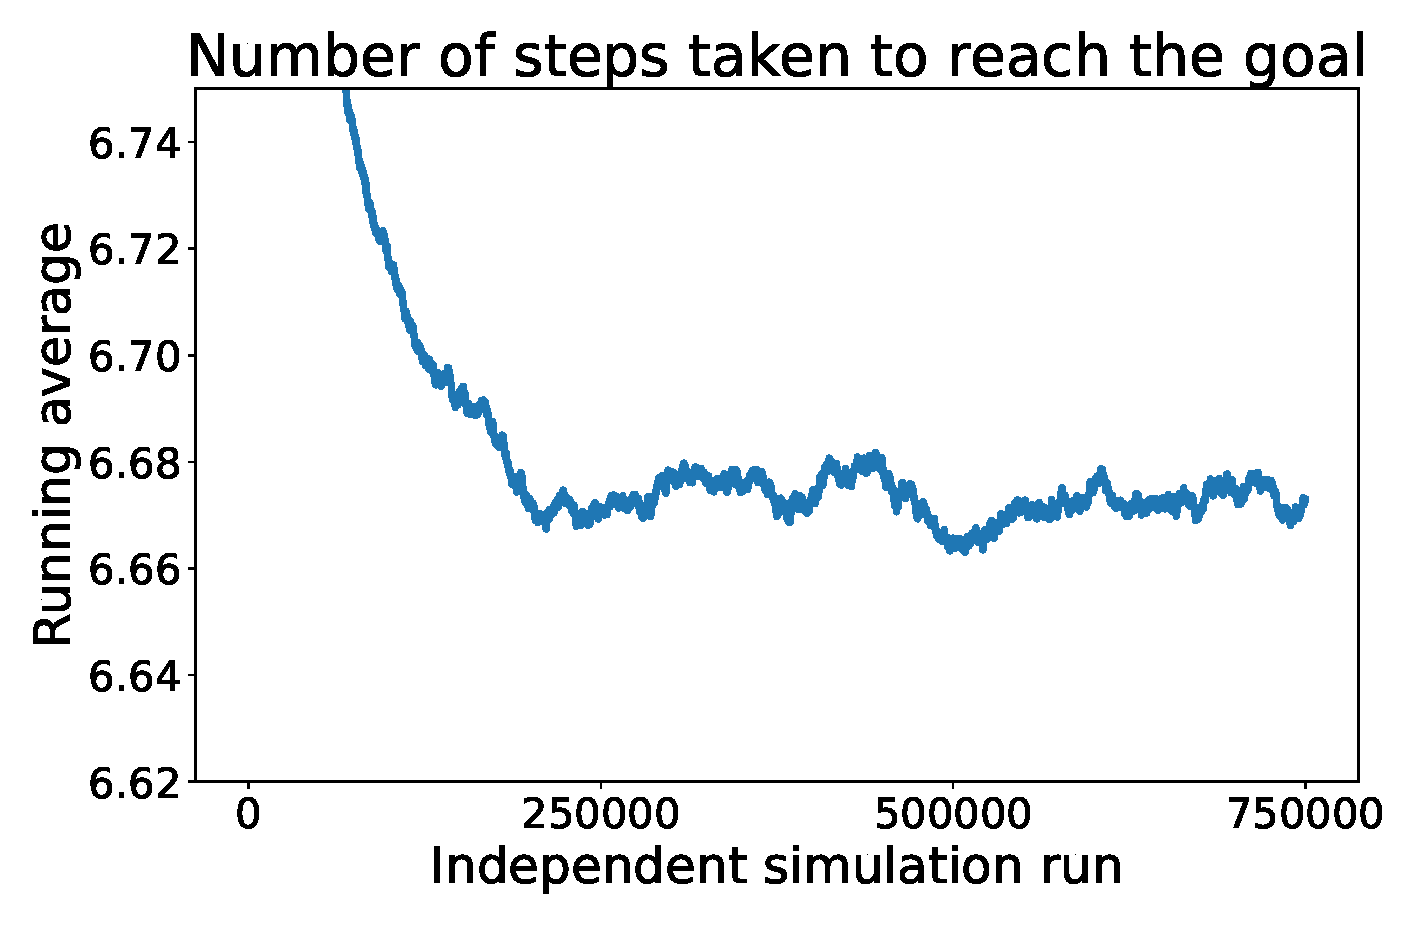
\includegraphics[width=0.5\textwidth]{./figures/running_avg.eps}
    \caption{Running average number of steps taken to reach the goal over $10,000$ independent Monte Carlo simulation runs.}
    \label{fig:running_avg}
\end{figure}
%
Figure~\ref{fig:running_avg} shows that the running average converges to $6.\bar{6}$ just as the theoretical computation indicated in Section~\ref{ssec:prob_sol}.

Figure~\ref{fig:histogram} shows the histogram of number of steps it took to 
solve the environment over $10,000$ independent Monte Carlo simulation runs. We 
observe that it takes $4$ steps to solve the environment $16.\bar{6}\%$ of the time, $6$ steps $33.\bar{3}\%$ of the time, and $8$ steps $50\%$ of the time, yielding an expected value of 
%
\[
\frac{1}{6} \times 4 + \frac{1}{3} \times 6 + \frac{1}{2} \times 8 = \frac{20}{3} = 6.\bar{6}.
\]
%
\begin{figure}[tbh]
    \centering
    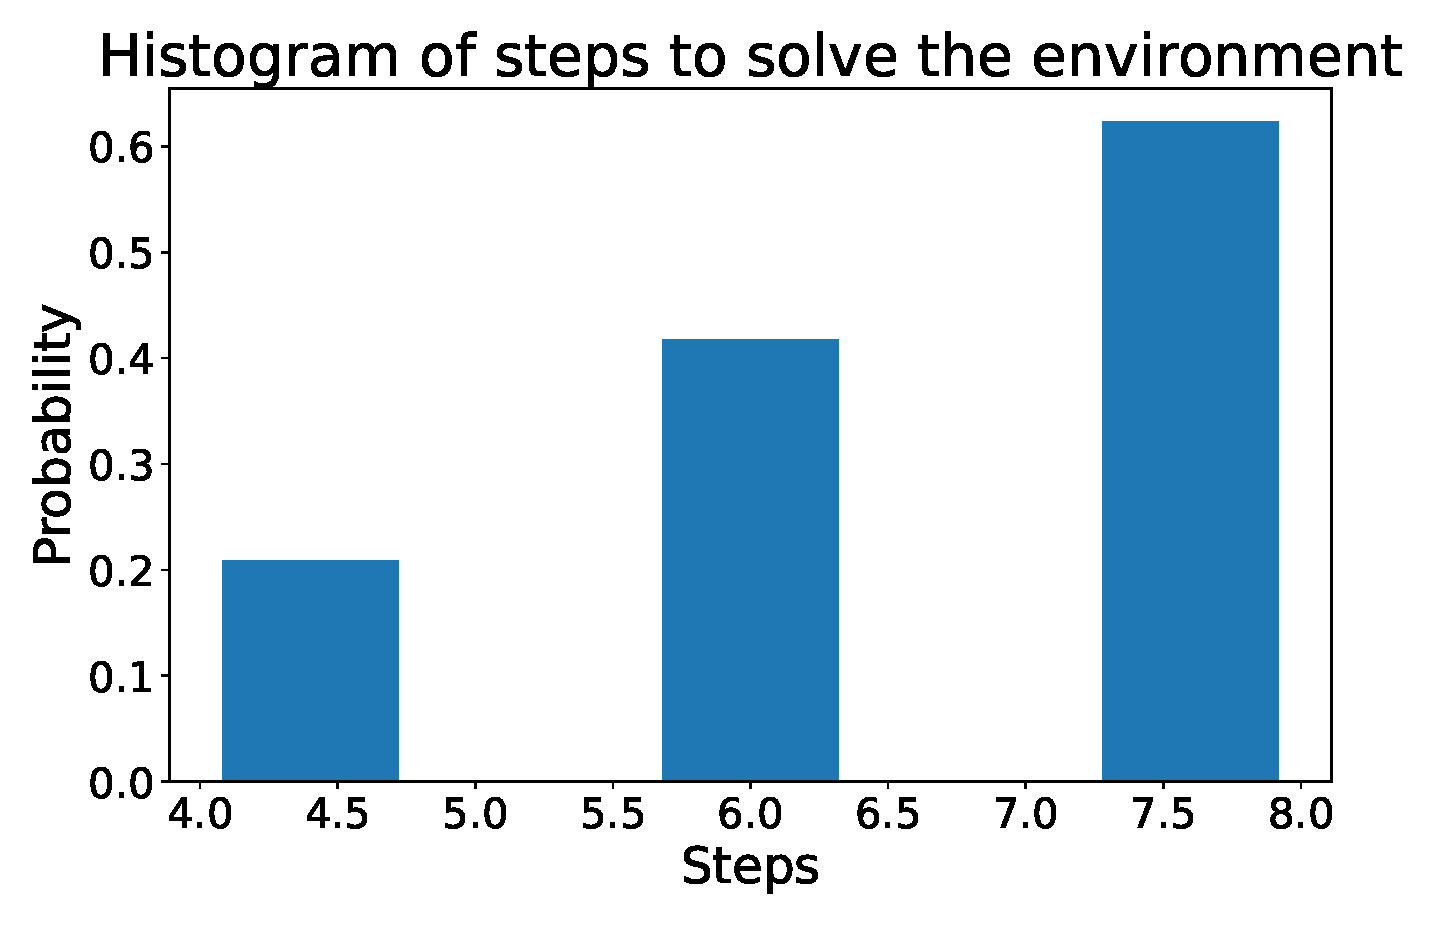
\includegraphics[width=0.5\textwidth]{./figures/steps_histogram.eps}
    \caption{Histogram of number of steps taken to solve the environment over $10,000$ independent Monte Carlo simulation runs.}
    \label{fig:histogram}
\end{figure}

The final Figure~\ref{fig:visit_count} shows the frequency of visits of each
state under the optimal policy deduced by $Q$-learning over $10,000$ independent
Monte Carlo runs.
%
\begin{figure}[bth]
    \centering
    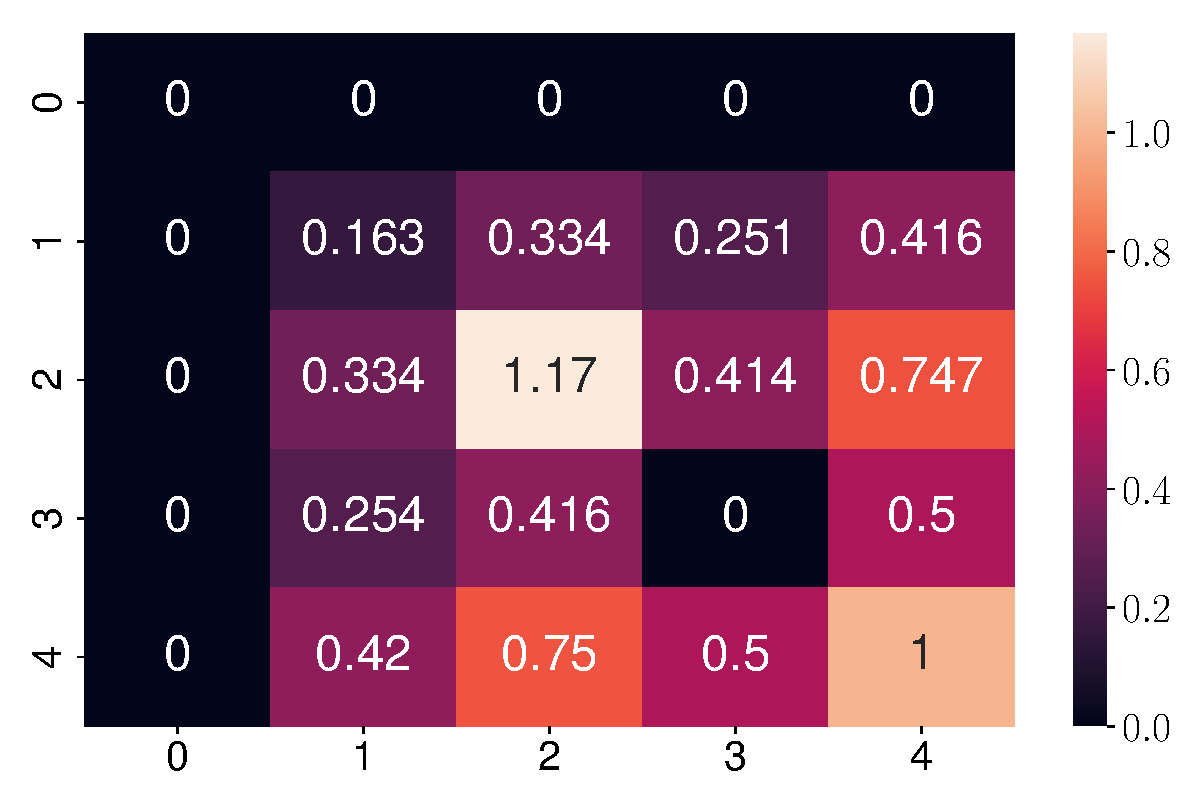
\includegraphics[width=0.5\textwidth]{./figures/visit_count.eps}
    \caption{Number of times a given state is visited under the optimal policy over $10,000$ independent Monte Carlo simulation runs.}
    \label{fig:visit_count}
\end{figure}
\section{Conclusions}
\label{sec:conclusion}
%
We have defined a novel grid world type optimal decision-making problem that is
meant to be solved by an RL agent in a one-shot manner. After thoroughly
defining the problem, we solved it theoretically with classical probability 
theory and then provided its RL formulation before running $Q$-learning to solve
it numerically.

The results of the RL solution is presented in Section~\ref{sec:experiment}. 
First observation was that the RL algorithm figures out the optimal policy in a
single episode, which gives same expected number of steps to reach the goal as
we find theoretically. This expected number is found by performing $50,000$
independent Monte Carlo simulation runs. Secondly, we have extracted additional 
statistics using these independent Monte Carlo runs. We have computed the 
distribution of the number steps it takes to reach the goal under the optimal 
policy, from which the expectation may be computed directly. We provided a 
distribution of the number of times all the states of the sibling grid world 
is visited. We also provided a plot of the scores of the bandit arms over the 
learning process (one-shot).

It is seen that one-shot RL may be performed in this simple, yet interesting
environment by learning two $Q$-functions in parallel. In this note, we used the
classical $Q$-learning algorithm. Other classical approaches such as double
$Q$-learning, etc. may be attempted and compared against our results here.


%% The Appendices part is started with the command \appendix;
%% appendix sections are then done as normal sections
%% \appendix

\clearpage
\bibliographystyle{elsarticle-harv}
% \biboptions{authoryear}
\bibliography{./bib/main}

\end{document}
